\documentclass[a4paper, twocolumn]{article}
\usepackage{booktabs}

%%%%%%%%%%%%%%%%%%%%%%%%%%%%%%%%%%%%%%%%%%%%%%%%%%%%%%%%%%%%%%%%%%%%%%%%%%%%%%
%%%%%%%%%  DO NOT EDIT !
%%%%%%%%%  DO NOT EDIT !
%%%%%%%%%  DO NOT EDIT !
%%%%%%%%%  DO NOT EDIT !
%%%%%%%%%  DO NOT EDIT !
%%%%%%%%%  DO NOT EDIT !
%%%%%%%%%%%%%%%%%%%%%%%%%%%%%%%%%%%%%%%%%%%%%%%%%%%%%%%%%%%%%%%%%%%%%%%%%%%%%%

\usepackage[english]{babel}
\usepackage{graphicx}             
\usepackage{tabularx}             
\usepackage{multirow}             
\usepackage{url}                 
\usepackage[ansinew]{inputenc}
\usepackage[small,bf]{caption}   
\usepackage{parskip}
\usepackage{amsmath}             
\usepackage{xcolor}
\usepackage{lipsum} 
 
%%%%%%%%%%%%%%%%%%%%%%%%%%%%%%%%%%%%%%%%%%%%%%%%%%%%%%%%%%%%%%%%%%%%%%%%%%%%%%
% fonts
%%%%%%%%%%%%%%%%%%%%%%%%%%%%%%%%%%%%%%%%%%%%%%%%%%%%%%%%%%%%%%%%%%%%%%%%%%%%%%

\usepackage{mathptmx}


%%%%%%%%%%%%%%%%%%%%%%%%%%%%%%%%%%%%%%%%%%%%%%%%%%%%%%%%%%%%%%%%%%%%%%%%%%%%%%
% spacing and indents
%%%%%%%%%%%%%%%%%%%%%%%%%%%%%%%%%%%%%%%%%%%%%%%%%%%%%%%%%%%%%%%%%%%%%%%%%%%%%%

\setlength{\parskip}{2pt}

%%%%%%%%%%%%%%%%%%%%%%%%%%%%%%%%%%%%%%%%%%%%%%%%%%%%%%%%%%%%%%%%%%%%%%%%%%%%%%
% geometry
%%%%%%%%%%%%%%%%%%%%%%%%%%%%%%%%%%%%%%%%%%%%%%%%%%%%%%%%%%%%%%%%%%%%%%%%%%%%%%

\usepackage[left=1.7cm,right=1.7cm,top=2.5cm,bottom=2.5cm]{geometry}
\setlength{\columnsep}{0.6cm}

%%%%%%%%%%%%%%%%%%%%%%%%%%%%%%%%%%%%%%%%%%%%%%%%%%%%%%%%%%%%%%%%%%%%%%%%%%%%%%
% make a header
%%%%%%%%%%%%%%%%%%%%%%%%%%%%%%%%%%%%%%%%%%%%%%%%%%%%%%%%%%%%%%%%%%%%%%%%%%%%%%

\usepackage{fancyhdr}
 
\pagestyle{fancy} 
\fancyhf{}  
\fancyhead[L]{\small\itshape Proceedings of the $9^{th}$ Conference on Interdisciplinary Musicology -- CIM14.
Berlin, Germany 2014}  
\fancyhead[C]{}  
\fancyhead[R]{}  
\renewcommand{\headrulewidth}{0.0pt}  
\fancyfoot[C]{}  
\renewcommand{\footrulewidth}{0.0pt}  

\pagestyle{fancy}

\makeatletter
\let\ps@plain\ps@fancy 
\makeatother
 
%%%%%%%%%%%%%%%%%%%%%%%%%%%%%%%%%%%%%%%%%%%%%%%%%%%%%%%%%%%%%%%%%%%%%%%%%%%%%%
% adjust titles
%%%%%%%%%%%%%%%%%%%%%%%%%%%%%%%%%%%%%%%%%%%%%%%%%%%%%%%%%%%%%%%%%%%%%%%%%%%%%%

\usepackage{titlesec}
  
\titleformat{\section}{\centering\normalfont\bfseries\sc\fontsize{10}{10}\selectfont}{\thesection.}{0.5em}{}
\titleformat{\subsection}{\normalfont\itshape\fontsize{10}{10}\selectfont}{\thesubsection.}{0.5em}{}
  
\titlespacing{\section}{0pt}{9pt}{2pt}
\titlespacing{\subsection}{0pt}{5pt}{0pt}
 
%%%%%%%%%%%%%%%%%%%%%%%%%%%%%%%%%%%%%%%%%%%%%%%%%%%%%%%%%%%%%%%%%%%%%%%%%%%%%%
% Strongly discourage hyphenation
%%%%%%%%%%%%%%%%%%%%%%%%%%%%%%%%%%%%%%%%%%%%%%%%%%%%%%%%%%%%%%%%%%%%%%%%%%%%%%

\hyphenpenalty=5000
\tolerance=1000

%%%%%%%%%%%%%%%%%%%%%%%%%%%%%%%%%%%%%%%%%%%%%%%%%%%%%%%%%%%%%%%%%%%%%%%%%%%%%%
% hyperref
%%%%%%%%%%%%%%%%%%%%%%%%%%%%%%%%%%%%%%%%%%%%%%%%%%%%%%%%%%%%%%%%%%%%%%%%%%%%%%

\usepackage{hyperref}

\hypersetup{
     unicode=false,           
    pdftoolbar=true,        
    pdfmenubar=true,        
    pdffitwindow=false,      
    pdfstartview={FitH},     
    pdftitle={},     
    pdfauthor={},      
    pdfsubject={},   
    pdfcreator={},   
    pdfproducer={},  
    pdfkeywords={keyword1} {key2} {key3}, 
    pdfnewwindow=true,      
    colorlinks=true,        
    linkcolor=darkgray,          
    citecolor=darkgray,         
    filecolor=darkgray,      
    urlcolor=darkgray            
}

%%%%%%%%%%%%%%%%%%%%%%%%%%%%%%%%%%%%%%%%%%%%%%%%%%%%%%%%%%%%%%%%%%%%%%%%%%%%%%
% abstract settings
%%%%%%%%%%%%%%%%%%%%%%%%%%%%%%%%%%%%%%%%%%%%%%%%%%%%%%%%%%%%%%%%%%%%%%%%%%%%%%
 
\newcommand{\CIMabstract}
[1]
{
\paragraph*{\itshape Abstract:} 
{ \bfseries
\fontsize{8}{9}\selectfont
#1
%
}
\vspace{0.3cm}}

 

 
\begin{document}

\fontsize{9}{9.5}\selectfont
 
%%%%%%%%%%%%%%%%%%%%%%%%%%%%%%%%%%%%%%%%%%%%%%%%%%%%%%%%%%%%%%%%%%%%%%%%%%%%%%
% THE TITLE
%%%%%%%%%%%%%%%%%%%%%%%%%%%%%%%%%%%%%%%%%%%%%%%%%%%%%%%%%%%%%%%%%%%%%%%%%%%%%%

\date{}                     

\title{\vspace{-8mm}\textbf{\sc%
\fontsize{16}{16}\selectfont
%
Haptic pattern representation using music technologies
%
\mbox{}\vspace{-1mm}
%
}}

%%%%%%%%%%%%%%%%%%%%%%%%%%%%%%%%%%%%%%%%%%%%%%%%%%%%%%%%%%%%%%%%%%%%%%%%%%%%%%
% AUTHORS
%%%%%%%%%%%%%%%%%%%%%%%%%%%%%%%%%%%%%%%%%%%%%%%%%%%%%%%%%%%%%%%%%%%%%%%%%%%%%%

\author{ %
%
Adam Tindale$^1$, Michael Cumming$^2$, Sara Diamond$^3$\\
%
 \textit{\normalsize %
$^1$ $^2$ $^3$ OCAD University Toronto, ON M5T 1W1 Canada
}\\
%
\footnotesize 
Correspondence should be addressed to: 
\href
{mailto:atindale@faculty.ocadu.ca}{atindale@faculty.ocadu.ca},
\href
{mailto:mcumming@ocadu.ca}{mcumming@ocadu.ca},
\href
{mailto:sdiamond@ocadu.ca}{sdiamond@ocadu.ca}
}

\maketitle
%
 
%%%%%%%%%%%%%%%%%%%%%%%%%%%%%%%%%%%%%%%%%%%%%%%%%%%%%%%%%%%%%%%%%%%%%%%%%%%%%%
% ABSTRACT
%%%%%%%%%%%%%%%%%%%%%%%%%%%%%%%%%%%%%%%%%%%%%%%%%%%%%%%%%%%%%%%%%%%%%%%%%%%%%%

\CIMabstract{
Wrist-wearable vibrotactile arrays can serve many functions: typically they are used for non-disruptive notification from social media. They can also be used for direction finding, gaming and entertainment. Authoring and programming of wrist-wearable vibrotactile arrays can be difficult because of the lack of standardized notational systems and file formats. Typically, each implementation of haptic arrays uses bespoke programming, which tends to isolate creative and technical development into non-communicating silos that discourage standardization and sharing. We propose that standard musical notation is an appropriate method for standardization and compositional expressiveness.
}

%%%%%%%%%%%%%%%%%%%%%%%%%%%%%%%%%%%%%%%%%%%%%%%%%%%%%%%%%%%%%%%%%%%%%%%%%%%%%%
% SECTIONS
%%%%%%%%%%%%%%%%%%%%%%%%%%%%%%%%%%%%%%%%%%%%%%%%%%%%%%%%%%%%%%%%%%%%%%%%%%%%%%

\section{Introduction}

We are developing a midi-driven, wrist-wearable device that integrates with a gaming app on an accompanying smartphone. The wrist device includes LED lights, vibe motors, buttons that activate when vibe motors are touched. It is controlled by a Bluetooth-enabled (low energy) LightBlue Bean microprocessor with a 3-axis accelerometer. This device combines several functions, including the control of gameplay from a smartphone or tablet, visual display of user's heart rate and interesting visual and vibrational patterns for entertainment and wearer adornment value \cite{tindale2014wearable}.\\

The game that is played on this device is a collections and discovery game for children aged 8-14 called \textit{Time Tremors} in which children collect crystals in order to unlock treasures that they then view on an accompanying smartphone app. Crystals are earned by the player through simple puzzle-solving, artifact discovery and physical activities. The end result is a sensory-intensive, transmedia game intended to encourage physical fitness and cultural exploration in children. On the device vibrotactile patterns play a major part and how to author patterns in a shareable and standardized way becomes an important consideration.\\

A wrist-wearable vibrotactile device, or what we call a 'vibe bracelet,' needs activation patterns to operate. It is unclear how to design such patterns in a standardized way using the technology closest at hand, which in our case is low-level code written in the C or Wiring languages. The design of vibe patterns for such devices is a specialized, yet multi-disciplinary area that straddles concerns for appropriate design of human computer interfaces suitable for wearables, and for potentially artistic patterns that look and feel attractive on the wrist.\\

Basic use cases for the wrist-wearable device include:
\begin{enumerate}
  \item Interpret wrist gestures and recognize overall physical activity of the wearer (using the \textit{Bean's} accelerometer),
  \item notify the wearer when crystals and treasures are earned,
  \item offer vibrotactile clues about where crystals and treasures can be found, and
  \item provide aesthetically attractive vibe and light displays corresponding to narrative points in a story.\\
\end{enumerate}

\begin{figure}[htb]
    \begin{center}
        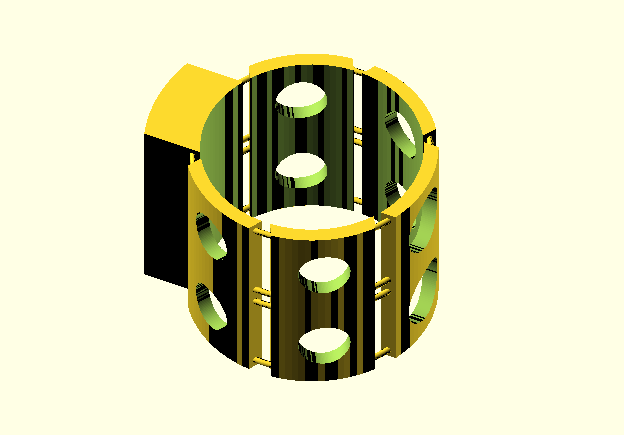
\includegraphics[width=0.4\textwidth]{graphics/bracelet-01.png}
    \end{center}
    \caption{Bracelet design [PRELIM].\label{fig:fig1}}
\end{figure}

It is the 3rd and 4th of these use cases that we consider for their potential musicality and the applicability of musical-inspired pattern design. We will do this by starting from basics and showing how we represent patterns, step by step.\\ 

\subsection{Vibrotactile clues}
They are intended to provide the following messages to the game-player:
such concepts as 'Go this way / don't go that way,'
'You're getting warmer / you're getting colder,' and 
'You're performing the correct movement / you're performing the wrong movement.'

The first two of these are spatial in nature and are also metaphorical, in that they refer to navigating through some kind of virtual space. The last one is kinesthetic in that it refers to moving your limbs through space in some preferred way.\\

Music does not lend itself, on first examination, to these sorts of concepts or metaphors. It is unclear at first what music that could be interpreted as 'go this way' might look like. 

\subsection{Basic conventions}
Our notational approach for our wrist-wearable device is to follow standard music notation (SMN) conventions and to see where these conventions lead us:

\begin{itemize}
\item Represent time horizontally form left to right: events to the right are later.
\item A note represents an activation of a component. A component can be of several types (vibe motor, LED, etc.). Place notes on normal, five line staves.
\item Represent note durations by note type (for example, quarter, half and whole notes), dots and by ties between notes of the same pitch.
\item If notes are pitched, indicate their pitch through their vertical placement on a staff. If notes are unpitched, represent different components (e.g. different types of vibe motors or LEDs) using various note heads or annotations.
\item Different \textit{parts} are on separate staves. One tactor type playing the same notes at the same time represents playing in \textit{unison}. For example, 48 tactors playing in unison can be represented as one part; there is no need to repeat the same information 48 times. 
\item Simultaneous notes, or \textit{chords} are stacked vertically, as in SMN.
\end{itemize}

%example here
As a second step we need to translate the nomenclature from our domain of vibrating wrist wearables to that of standard music. The flowing table indicates the mapping we have applied from our domain to that of music notation:

\begin{table}[htbp]
\caption{Vibrotactile vs Music notation terms}
\small
\centering
\begin{tabular}{@{}ll@{}}
\toprule
Vibrotactile term & SMN term \\ 
\midrule
Activation of one component & Note \\
Activation duration & Note duration \\
One type of component & Instrument \\
Series of activations for one instrument & Part \\
Frequency of an activation & Pitch \\
Simultaneous activations w/ multiple pitches & Chord \\ 
\bottomrule
\end{tabular}
\end{table}

\begin{figure}[htb]
    \begin{center}
        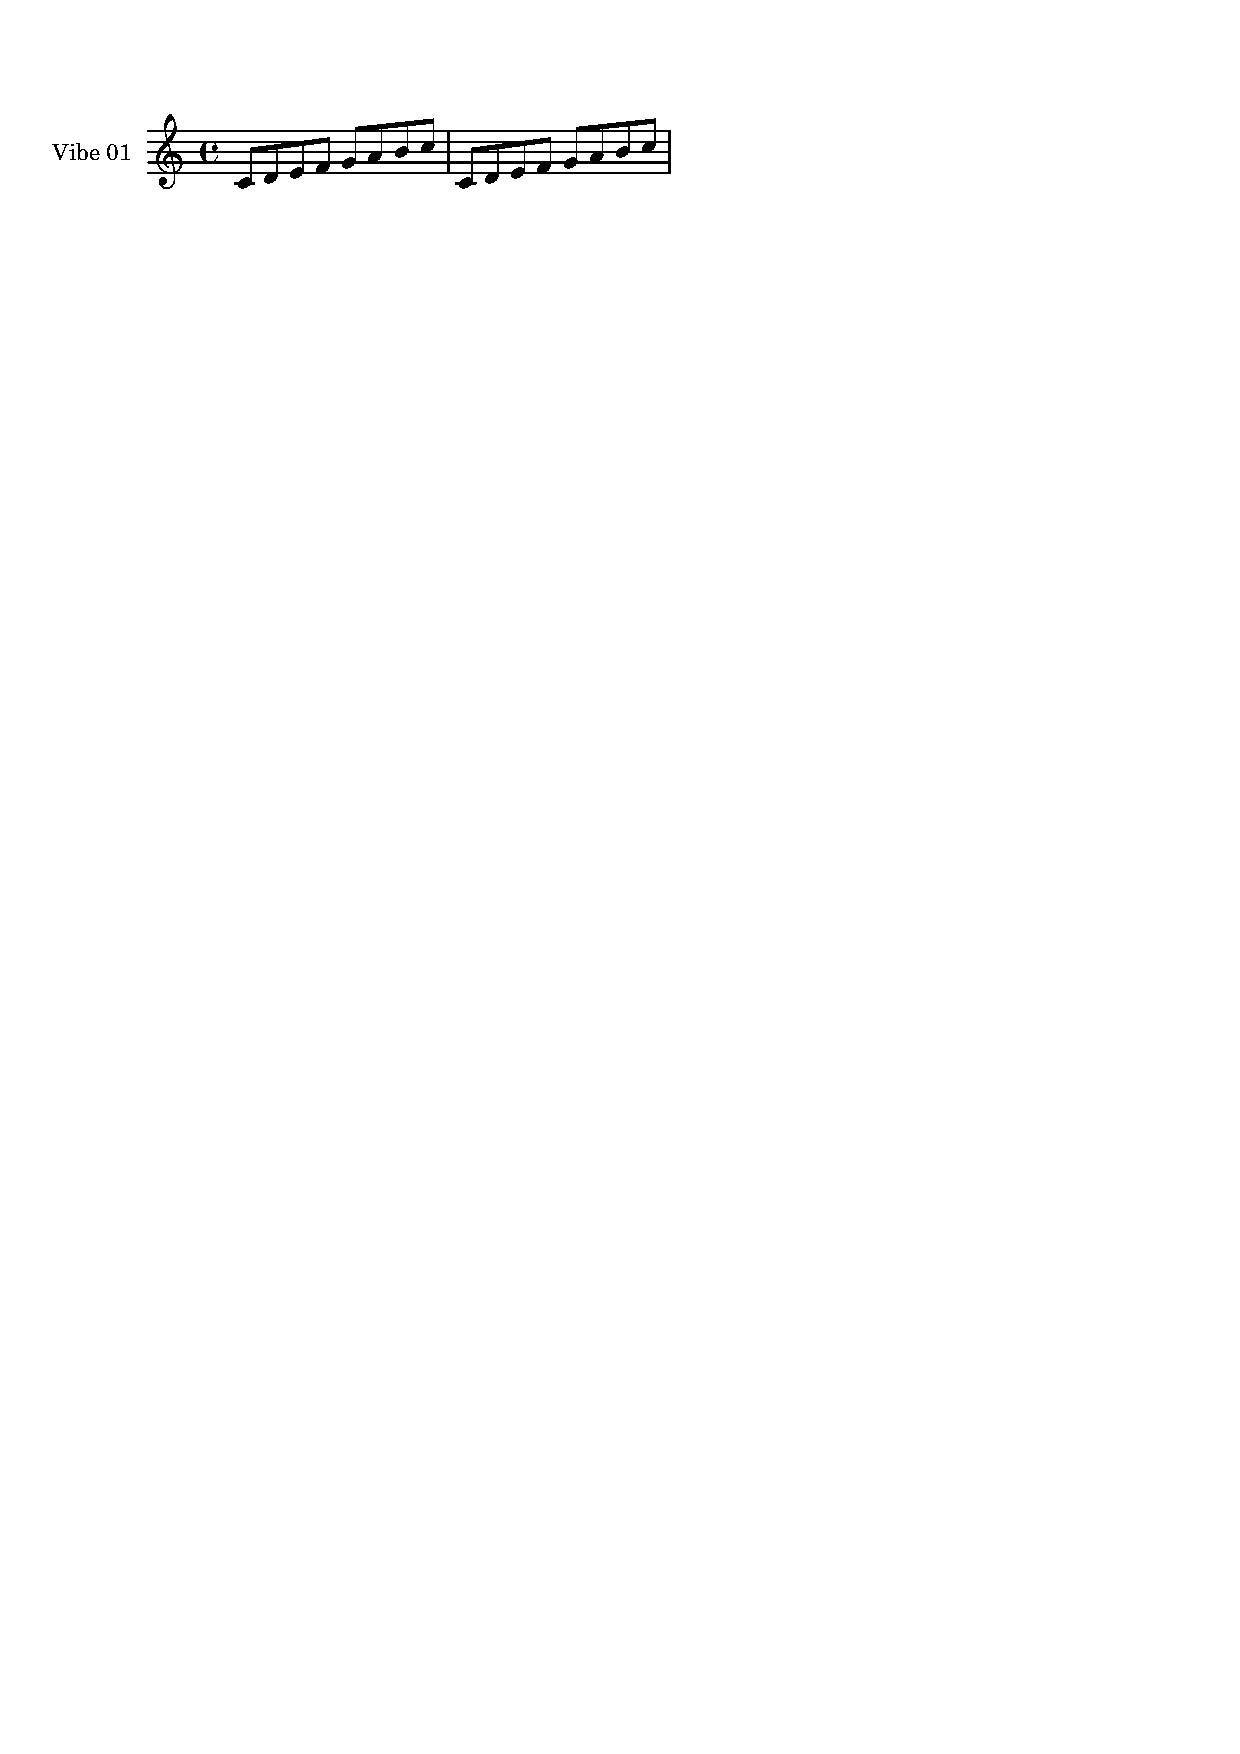
\includegraphics[width=0.4\textwidth]{graphics/scaleArduino-01.pdf}
    \end{center}
    \caption{Simple scale for a pitched Arduino component.\label{fig:fig2}}
\end{figure}

\begin{figure}[htb]
    \begin{center}
        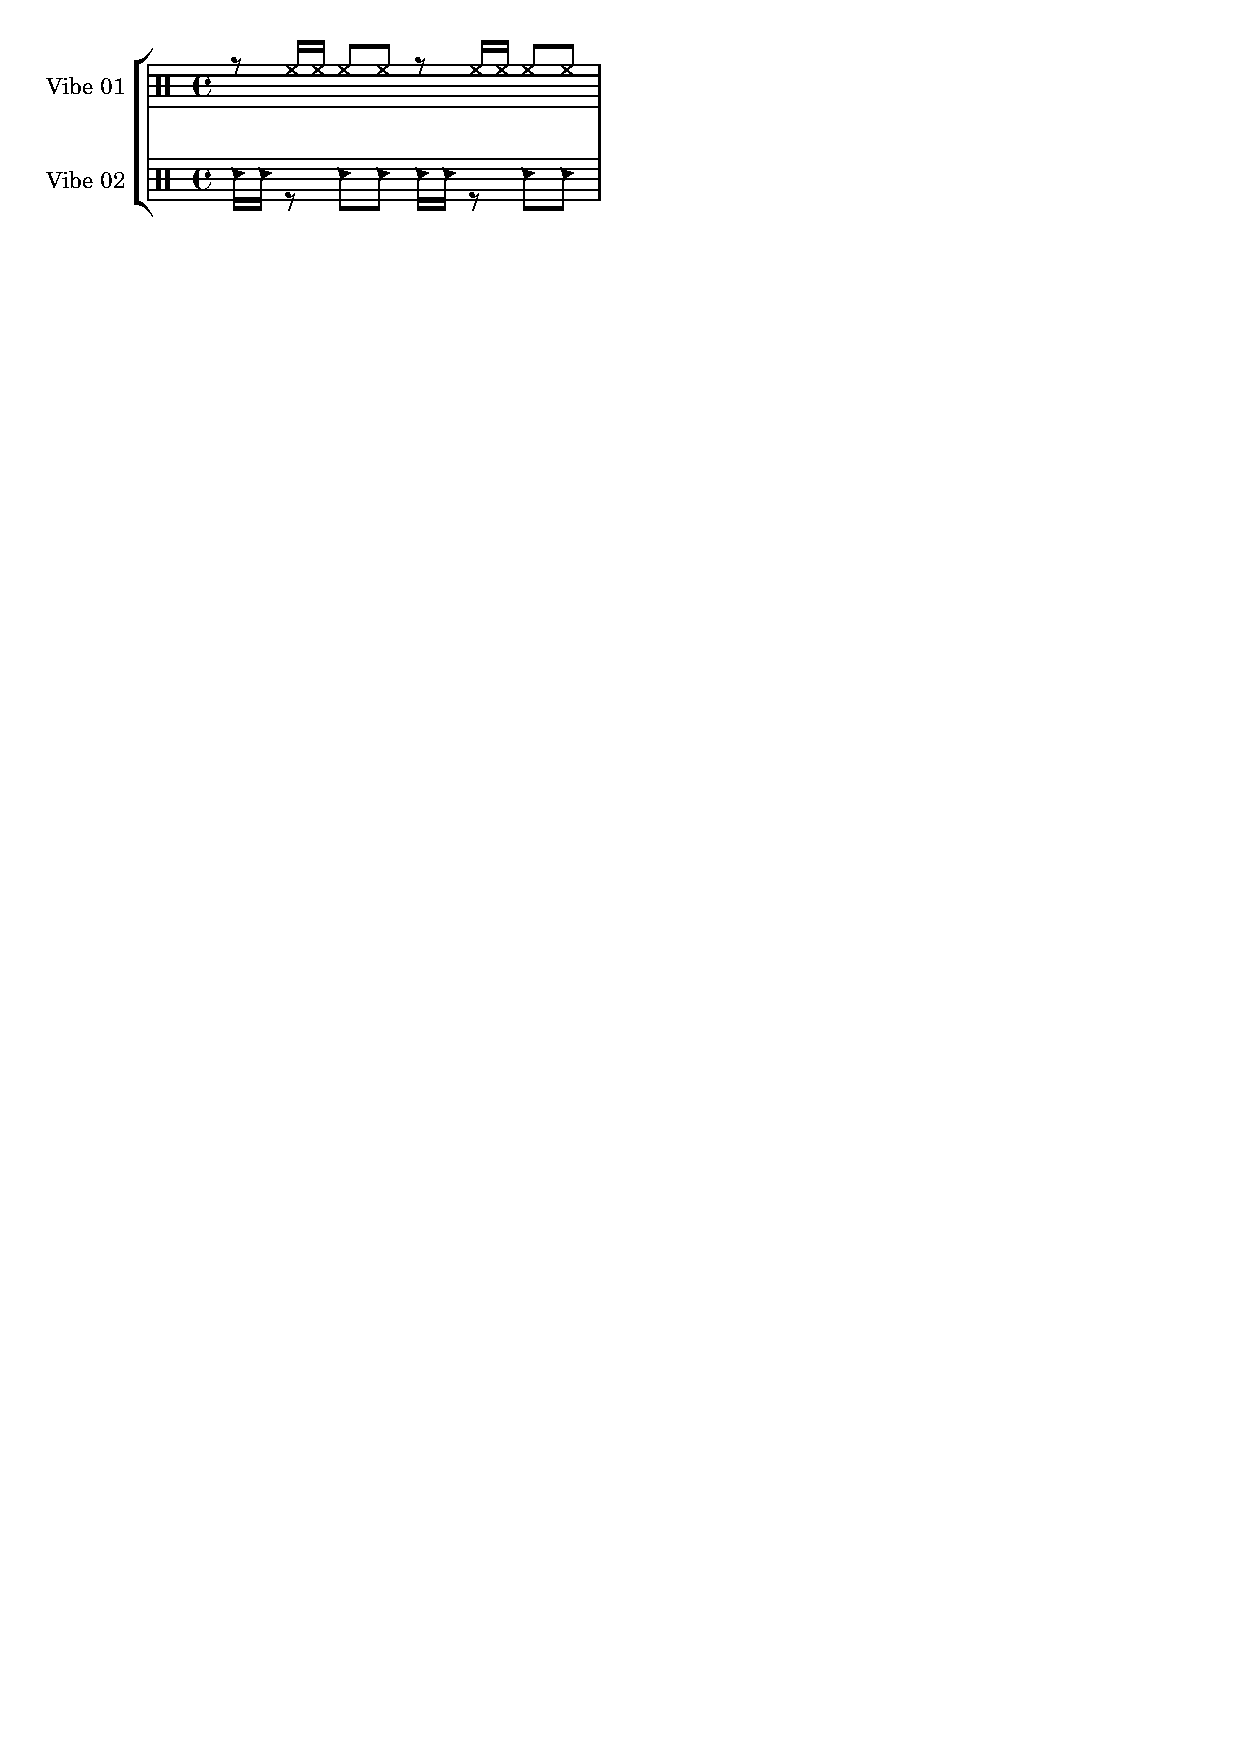
\includegraphics[width=0.4\textwidth]{graphics/drums1-simple.pdf}
    \end{center}
    \caption{Simple rhythm for two unpitched Arduino components.\label{fig:fig3}}
\end{figure}

\begin{figure}[htb]
    \begin{center}
        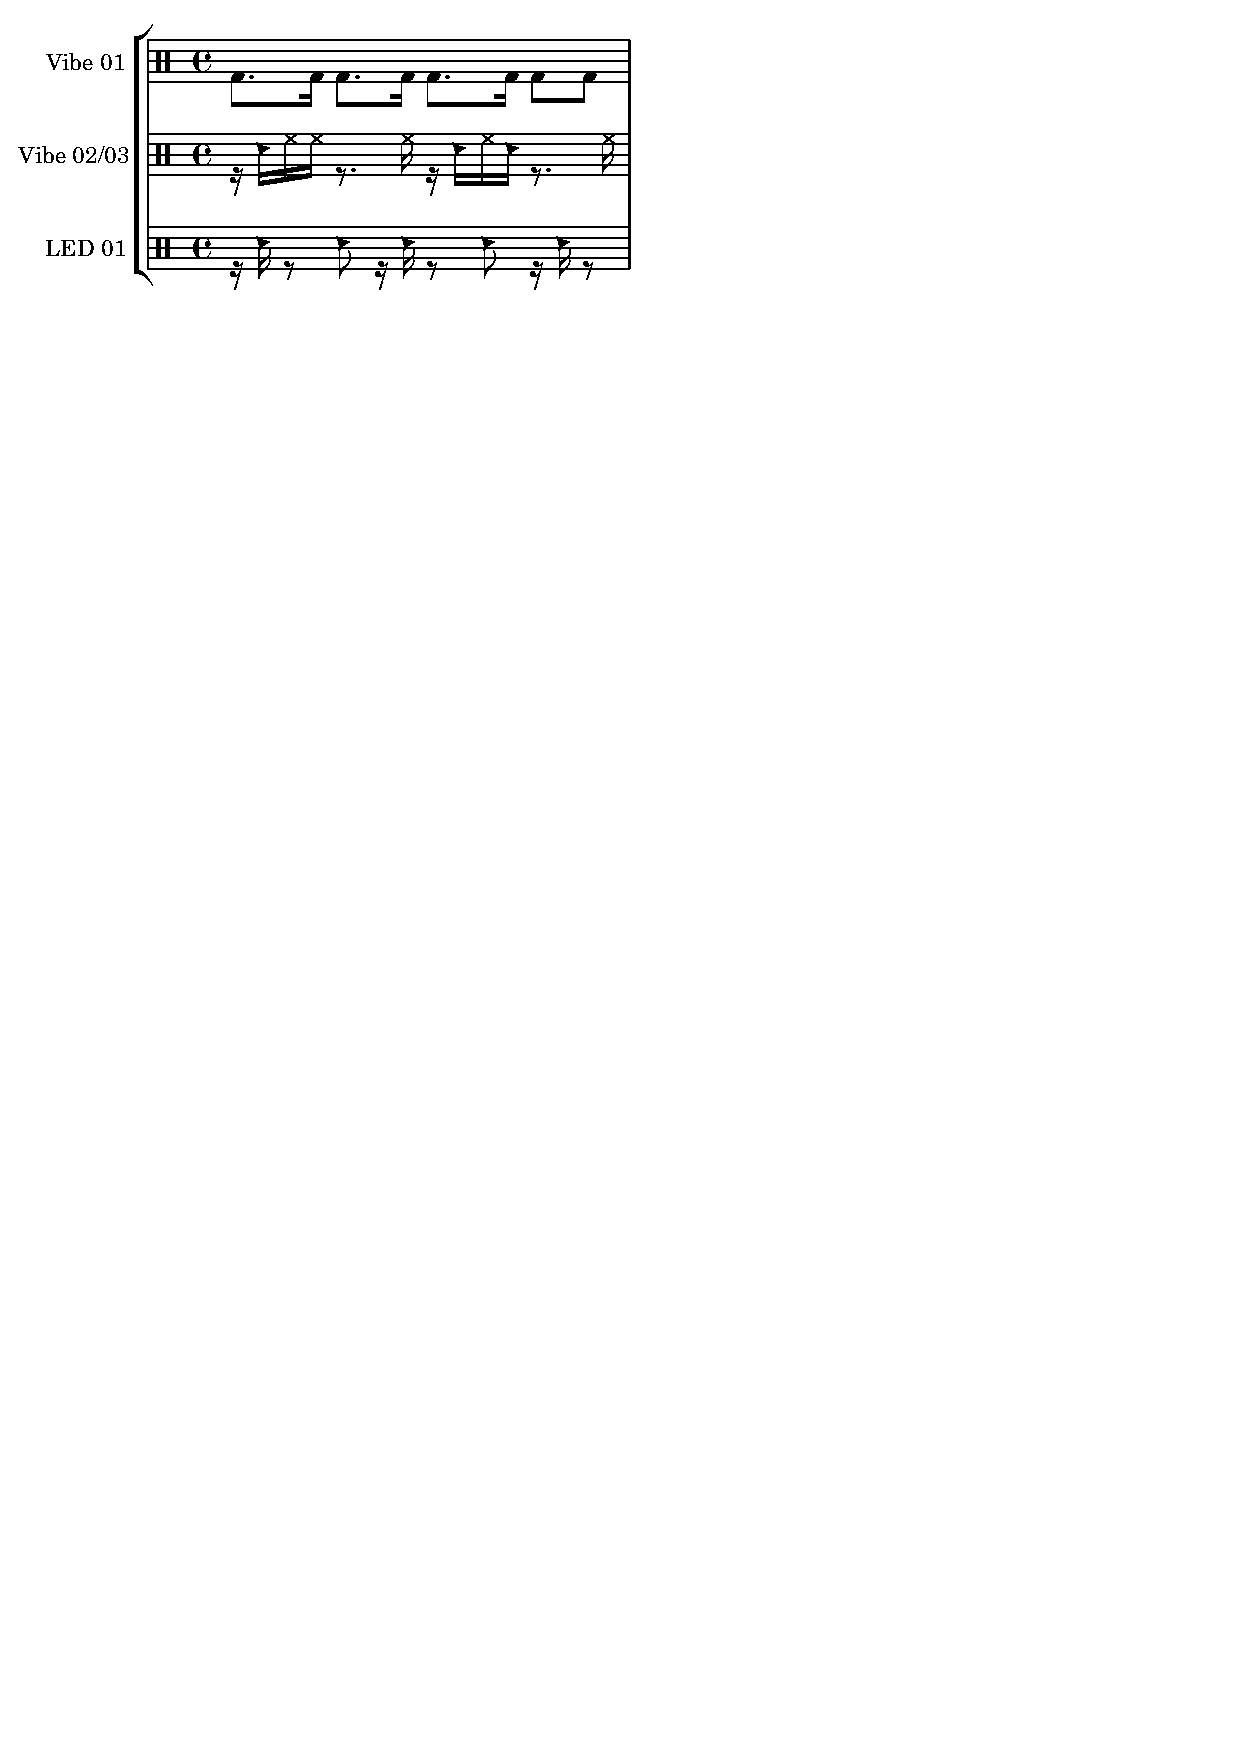
\includegraphics[width=0.4\textwidth]{graphics/drums1-multistaff.pdf}
    \end{center}
    \caption{Complex rhythm for three Arduino components.\label{fig:fig4}}
\end{figure}


Examples to show (in SMN):
simple: one part, no pitch, rhythm
more complex: two parts, pitched
complex: many parts, SATB style, melody line, rhythms

\subsection{Pitch}
Vertical placement for normal, pitched notes in SMN indicates their pitch. The pitch of a note is one of its primary psychoacoustic attributes, along with its duration, loudness and timbre. Unpitched notes are those for which the frequency is indeterminate, too complex or unrelated to the pitch contours of melodic or harmonic parts. The perception of pitch in vibrotactile devices differs from that of normal acoustic instruments. The number of frequency differences is much reduced and depends on amplitude. There may be as few as five frequency distinctions possible with cutaneous perception, or as many as ten \cite{van2003distilling}. The skin's maximal frequency response occurs around 250 Hz \cite{gunther2003cutaneous}. So it is clear that the chromatic range of pitches and frequencies over many octaves as normally represented using music notation is not suitable for cutaneous perception, but that some variation in pitch is possible. 

\subsection{Intensity}
As with aural music, suitable intensities for vibrotactile devices range from those that are barely perceptual to those that become uncomfortable. Considerations of the amplitude envelope (amplitude, delay, sustain, release, or ADSR) and with amplitude modulations such as tremolo or pitch modulations like vibrato \cite{gunther2003cutaneous}. 

\subsection{Duration}
If vibrotactile notes are of short duration they are perceived as sharp taps or jobs in the skin \cite{gunther2003cutaneous}. 


\section{Related Work}

\subsection{Haptic feedback and communication}
Haptic communication through force feedback is a common technique used in gaming. It purpose is to introduce the sense of touch to interactions such as movement through space, collision with, and proximity to, objects, and notification of awarding of game points and of proximity to dangerous situations. Touch can add sensual aspects and realism to computer interactions and may be useful in reducing sensory overloads from other perceptual modalities such those used in graphical interfaces \cite{oakley2000putting}, or with devices too small to have large visual displays.\\

Oakley provides a useful taxonomy of haptic-related terms, such as proprioceptive, kinesthetic and tactile. Haptic is a general term relating to the sense of touch, while tactile is more specific and relates to the sensation of pressure rather than that of temperature or pain \cite{oakley2000putting}. The largest organ of the human body is the skin and has great potential for the transmittal of information and sensation \cite{lindeman2006wearable} \cite{brewster2004tactons}.\\

Haptic feedback has a long history in the design of computer mice and of other hand controllers \cite{yang2005novel}. Touch is of course useful in generating intimacy in normal social situations \cite{bronner1982haptic}. It can also be used to coordinate action in online or gaming situations \cite{ho1998experiment}. The new Apple Watch also enables wearers to communicate their heartbeat to others wirelessly \cite{johnson2014literature}.\\

\subsection{Wearable vibrotactile devices}
Typically, haptic devices beyond experimental contexts are either wearable or holdable. One challenge of wearable devices is how to encourage people to wear them. People tend to be very particular about the look and feel of devices that provide potentially intimate notifications.\\ 

The purposes of such devices are varied and include emulation of attention-getting practices such as the squeezing of wrists, touching of shoulders and pats on arms. As Baumann notes, such social gestures may include a wealth of sub-texts including urgency, affection and reinforcement of social hierarchies \cite{baumann2010emulating}.\\

Due to their potentially non-disruptive nature, vibrotactile devices could aid in tasks in which the user's attention might be devoted to some other task, such as navigation, or gameplay, or in situations where visual information is scarce or non-existent, as with the blind \cite{ertan1998wearable}.  Devices vary in the degree of body contact they provide. The ability of he body to perceiver vibrotactile stimuli varies greatly between regions of the body dues to variation in skin receptor density \cite{lindeman2006wearable}. Work has been also done in wide-area stimulation instead of areas of the body where receptor density is greatest, such as the tips of the fingers and lips.\cite{lindeman2004towards}.


Vibrational patterns suitable for a wrist device are much less complex than those designed for auditory perception due to the constrained perceptual channel of the cutaneous and kinaesthetic possibilities of the wrist compared to that of our ears.\\  

\subsection{Pattern authoring for vibrotactile devices}
It is clear that appropriate patterns for vibrotactile devices depends on what you want such devices to do. It also depends of course on what the device is capable of doing. 

\section{Designing patterns for midi-driven vibe devices}

\subsection{Introduction}
One way of creating midi control patterns is to compose music in such a way that midi data describing the music is produced as a side-effect.

This, of course, is standard procedure in modern music production. One way of producing midi is by using the text-based music engraving and compositional tool Lilypond.\\

Vibrotactile clues tend to be rhythmic in nature. Like any other rhythm, these can, in theory, be represented in musical notation. Pitch differentials are also possible with tactors, as their frequency can be modelled using standard pulse-width modulation (PWM) techniques.\\

Therefore, the basic components of music are present even with a wrist-wearable vibrotactile device that does not, at first, seem to have a musical aspect: \textit{notes} with durations, pitched notes played on various discrete \textit{instruments} (vibe motors and LED lights), various \textit{parts,} or \textit{voices,} played in polyphonic \textit{compositions} and the dynamics of various parts playing together. As shown below the translation of these concepts into standard musical notation is fairly straightforward.\\

Requirements for vibe design on bracelets includes the ability to provide a means of designing tactor activation patterns in a standardized way, activate a tactor (vibe motor) individually (monophony) or simultaneously with various ?parts? (polyphony), have vibrations of specified durations, intensities and possibly pitches, and to activate rhythmic patterns over time.\\




Aspects that seem less musical in nature
Vibrotactile clues in our game are directional in nature. They point in specific directions and therefore have a spatial direction. 

\section{Discussion}
\section{Future Work}
\section{Conclusion}
\section{Acknowledgements}

%%%%%%%%%%%%%%%%%%%%%%%%%%%%%%%%%%%%%%%%%%%%%%%%%%%%%%%%%%%%%%%%%%%%%%%%%%%%%%
% REFERENCES
%%%%%%%%%%%%%%%%%%%%%%%%%%%%%%%%%%%%%%%%%%%%%%%%%%%%%%%%%%%%%%%%%%%%%%%%%%%%%%

\bibliography{CIM14_bibliography}
\bibliographystyle{CIM14}
  
\end{document}
